\documentclass[red]{beamer}
%\usetheme{Berkeley}
\usepackage{adjustbox}
\usepackage{graphicx}
\usepackage{wrapfig}
\usepackage{caption}
\captionsetup{justification=centering}
\graphicspath{ {images/} }
\setbeamertemplate{footline}[frame number]{}
\defbeamertemplate*{footline}{noslidenum theme}



\title{“Gerrymandering in the Laboratory”}
\author{SunAh An \and Buddy Anderson \and Cary Deck}
\institute{The University of Alabama}
\date{EC698 November 15, 2021}

%/ *****TITLE SLIDE*****
\begin{document}
\begin{frame}
\titlepage
\end{frame}





%/ *****Gerrymandering*****
    \section{Gerrymandering}
    \begin{frame} [t]
    \frametitle{What is gerrymandering?}
    \begin{itemize}
        \item The manipulation of the boundaries of electoral constituencies to favor one election outcome over another
        \item Etymology began in 1812 when Massachusetts Governor Elbridge Gerry, signed a bill redrawing state senate districts
    \end{itemize}
    \begin{columns}
    \begin{column}{0.45\textwidth}
    \begin{center}
    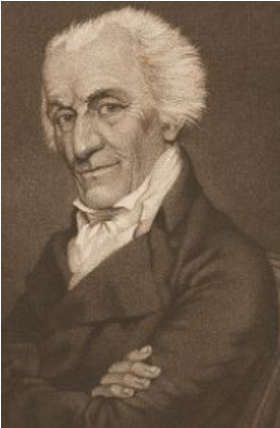
\includegraphics[scale = .40]{elbridge_gerry.png}
    \captionof*{figure}{Elbridge Gerry}
    \label{fig:gerry}
    \end{center}
    \end{column}
    \begin{column}{0.45\textwidth}
    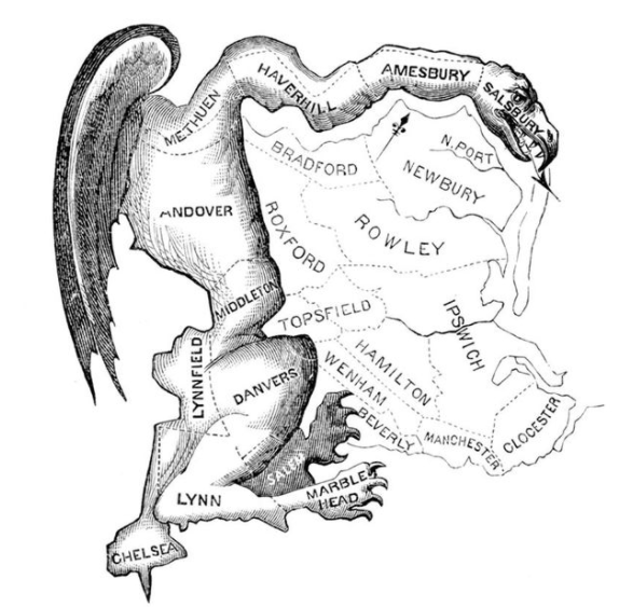
\includegraphics[scale = .40]{gerry_salamander.png}
    \captionof*{figure}{Gerry's Salamander}
    \label{fig:salamander}
    \end{column}
    \end{columns}
    \end{frame}

%/ *****Gerrymandering*****
    %\section{Gerrymandering}
    \begin{frame} [t]
    \frametitle{Examples of Gerrymandering}
    \begin{figure}[h]
    \begin{center}
    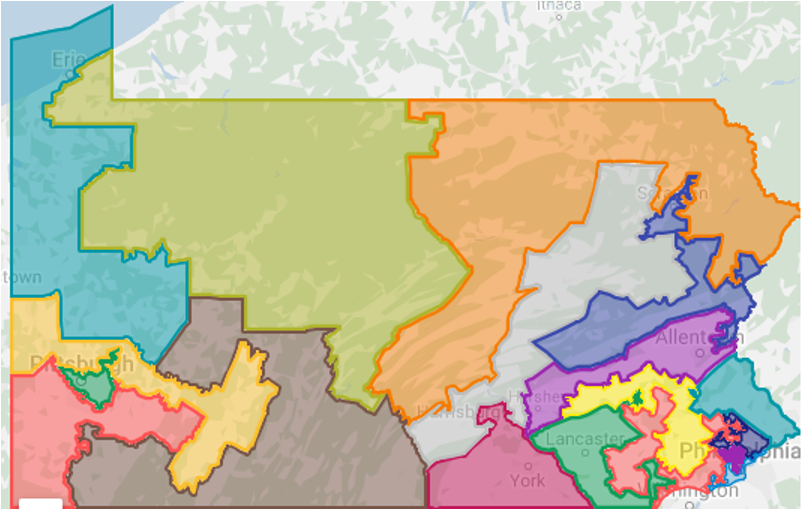
\includegraphics[scale=0.7]{PA_big.png}
    \captionof*{figure}{Pennsylvania's 18 Congressional Districts}
    \label{fig:PA_big}
    \end{center}
    \end{figure}  
    \end{frame}
    
%/ *****Gerrymandering*****
    %\section{Gerrymandering}
    \begin{frame} [t]
    \frametitle{Examples of Gerrymandering}
    \begin{figure}[h]
    \begin{center}
    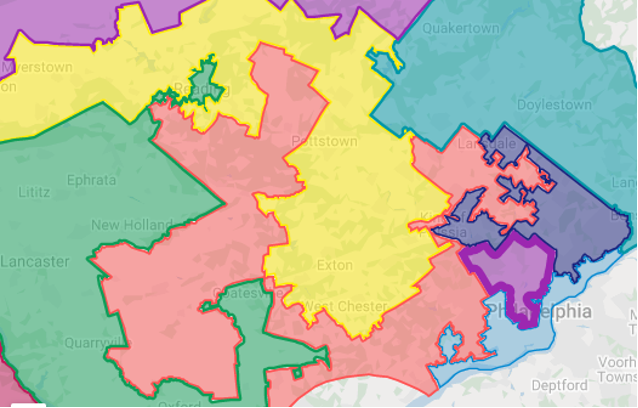
\includegraphics[scale=0.75]{PA_small.png}
    \captionof*{figure}{Pennsylvania's $7^{th}$: Goofy kicking Donald}
    \label{fig:PA_small}
    \end{center}
    \end{figure}  
    \end{frame}
    
%/ *****Gerrymandering*****
    %\section{Gerrymandering}
    \begin{frame} [t]
    \frametitle{Alabama Congressional Districts}
    \begin{columns}
    \begin{column}{0.45\textwidth}
    AL is 25\% African-American
    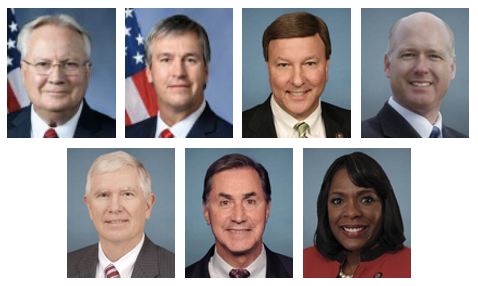
\includegraphics[scale = .62]{AL_reps.png}
    \captionof*{figure}{AL Representatives}
    \label{fig:AL_reps}
    \end{column}
    \begin{column}{0.40\textwidth}
    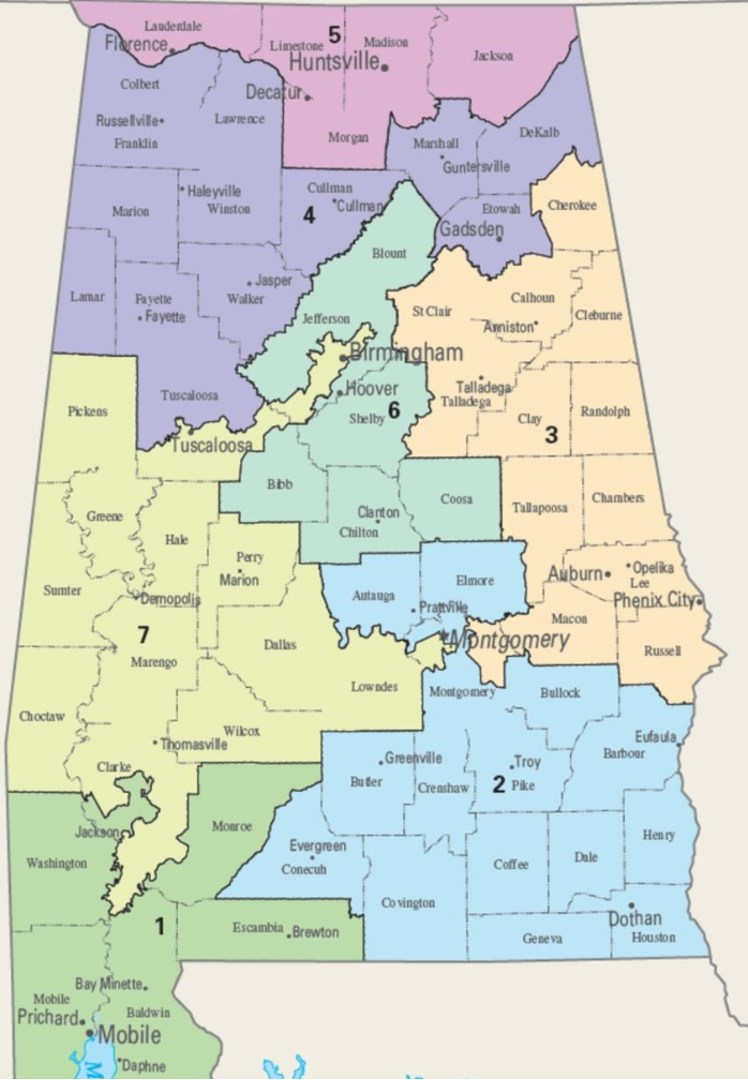
\includegraphics[scale = .30]{AL_electoral_map.png}
    \captionof*{figure}{AL Districts}
    \label{fig:AL_districts}
    \end{column}
    \end{columns}
    \end{frame}

%/ *****Gerrymandering*****
    %\section{Gerrymandering}
    \begin{frame} [t]
    \frametitle{Cracking and Packing}
    \begin{itemize}
        \item Cracking refers to spreading supports across districts.
        \item Packing refers to concentrating the rival’s supporters into a few districts.
    \end{itemize}
    \begin{columns}
    \begin{column}{0.35\textwidth}
    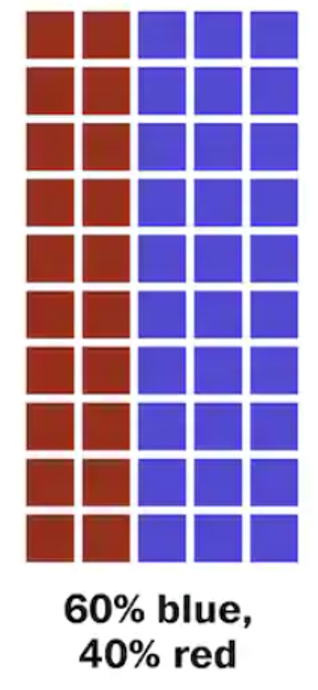
\includegraphics[scale = .5]{example_crack_and_pack.png}
    \end{column}
    \begin{column}{0.35\textwidth}
    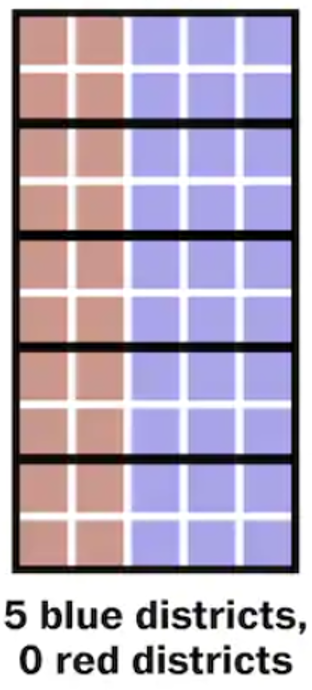
\includegraphics[scale = .5]{cracking.png}
    \end{column}
    \begin{column}{0.35\textwidth}
    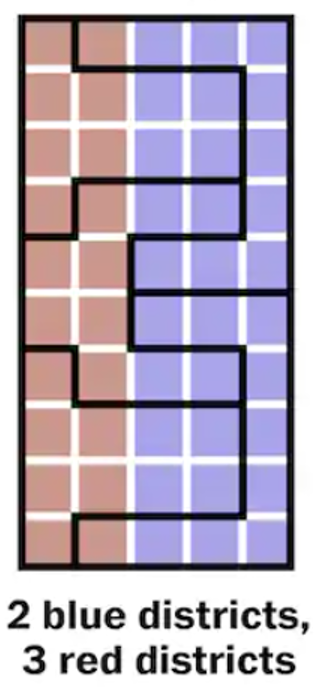
\includegraphics[scale = .5]{packing.png}
    \end{column}
    \end{columns}
    \end{frame}

%/ *****Previous work on Gerrymandering*****
    \section{Literature Review}
    \begin{frame} [t]
    \frametitle{Literature Review}
    \begin{itemize}
        \item Optimal Gerrymandering
            \begin{itemize}
                \item Two types of voters (Owen and Grofman 1988) 
                \item Continuum of perfectly observable types (Gilligan and Matsusaka 1999)
                \item Imperfectly observable types (Friedman and Holden 2008; Gul and Pseendorfer 2010; Kolotilin and Wolitzky 2020)
            \end{itemize}
        \item Implications of Gerrymandering
            \begin{itemize}
                \item Majority minority districts (Cameron, Epstein and O’Halloran 1996; Grigg and Katz 2005)
                \item Participation (Hayes and McKee 2009)
                \item Policy choice (Shots 20002; Besley and Preston 2007)
                \item Polarization (McCarty, Pool, and Rosenthal 2009)
            \end{itemize}
    \end{itemize}
    \end{frame}

%/ *****Theory*****
    \section{Theory}
    \begin{frame}[t]
    \frametitle{Our Contest Map}
    \begin{itemize}
        \item A Map consists of 3 Districts that each contain 3 Zones
        \item Players A and B compete for a prize of $V$ by choosing expenditures for each District
        \item To win a District a player must win a majority of the Zones in that District
        \item To win the contest a player must win the majority of the Districts
        \item Zones are either predetermined or competitive
        \item Competitions at the Zone level are determined by Tullock Contests based on District expenditure
    \end{itemize}
    \end{frame}

%/ *****Theory*****
    \begin{frame} [t]
    \frametitle{Our Contest Map}
    \begin{center}
    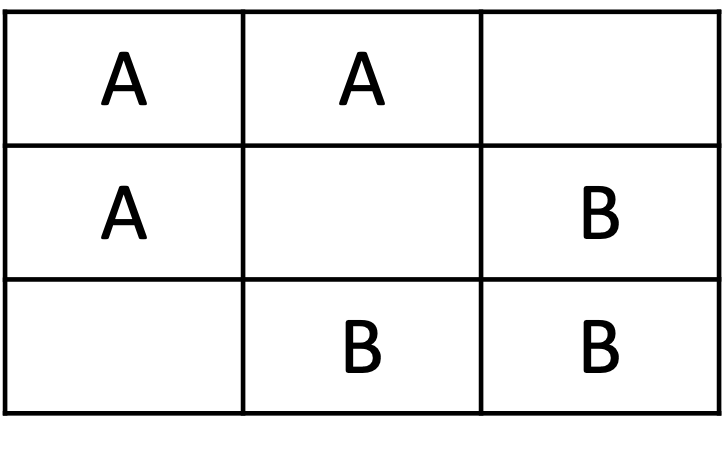
\includegraphics[width=0.25\textwidth]{blank_map.png}
    \end{center}
    \begin{itemize}
        \item There are 3 predetermined Zones for each player
        \item Districts are referenced by their color: White, Light Gray, and Dark Gray
        %Any other map that could be constructed with  three  zones  of  three  districts  each  where  one  third  of  the  zones  are  not preassigned and the other districts are equally split between the two players is strategically equivalent to one of these five maps.
        \item Maps are either (Gerry)mandered or (Symm)etric
    \end{itemize}
    \vspace{0.4cm}
    \begin{columns}
    \begin{column}{0.15\textwidth}
    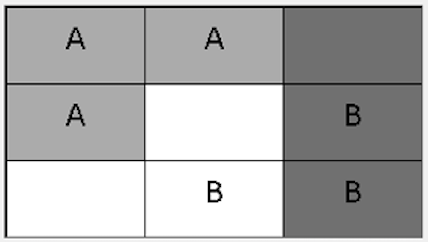
\includegraphics[scale = .25]{Gerry_B.png}
    \captionof*{figure}{$Gerry_B$}
    \end{column}
    \begin{column}{0.15\textwidth}
    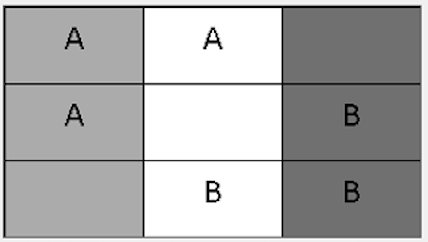
\includegraphics[scale = .25]{Symm_1_1.png}
    \captionof*{figure}{$Symm_{1,1}$}
    \end{column}
    \begin{column}{0.15\textwidth}
    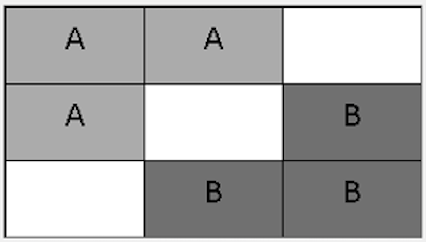
\includegraphics[scale = .25]{Symm_1_3.png}
    \captionof*{figure}{$Symm_{1,3}$}
    \end{column}
    \begin{column}{0.15\textwidth}
    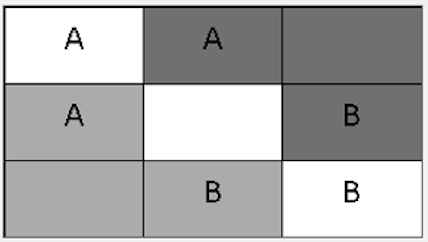
\includegraphics[scale = .25]{Symm_3_1.png}
    \captionof*{figure}{$Symm_{3,1}$}
    \end{column}
    \begin{column}{0.15\textwidth}
    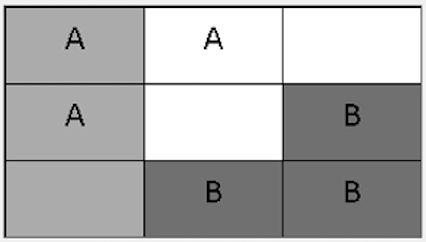
\includegraphics[scale = .25]{Gerry_A.png}
    \captionof*{figure}{$Gerry_A$}
    \end{column}
    \end{columns}
    \end{frame}
    
%/ *****Theory*****
    \begin{frame} [t]
    \frametitle{Theoretical Predictions}
    \begin{itemize}
        \item Player $i$'s expected payoff is $E\pi_i = \rho_i V - \sum_{d} e_{i,d|M}$ for
        \begin{itemize}
            \item the probability $\rho_i$ that player $i$ wins the Map and
            \item the expenditure $e_{i,d|M}$ of player $i$ in district $d$ on the given Map $M$
        \end{itemize}
    \end{itemize}
    \begin{columns}
    \begin{column}{0.25\textwidth}
    \begin{center}
    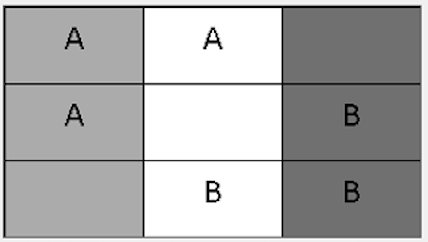
\includegraphics[scale = .4]{Symm_1_1.png}
    \captionof*{figure}{$Symm_{1,1}$}
    \end{center}
    \end{column}
    \begin{column}{0.6\textwidth}
    \begin{itemize}
        \item Player A wins District L \Rightarrow $e_{A,L}^* = e_{B,L}^* = 0$
        \item Player B wins District G \Rightarrow $e_{A,G}^* = e_{B,G}^* = 0$
        \item The winner of District W wins the contest
        \item Standard Tullcok Contest for lone, unclaimed Zone in White District
        \begin{itemize}
            \item $e_{A,W}^* = e_{B,W}^* = \frac{V}{4}$
            \item Both players have 50\% chance of winning
        \end{itemize}
    \end{itemize}
    \end{column}
    \end{columns}
    \end{frame}

%/ *****Theory*****
    \begin{frame} [t]
    \frametitle{Theoretical Predictions}
    \begin{table}[ht]
    \centering 
    \label{tabeq}
    \begin{tabular}{c c c c c c} 
    \hline\hline\\[-1.8ex]
        Map & District & $e_{A|M}^*$ & $e_{B|M}^*$ & $\rho_A$ & $\rho_B$ \\ [0.5ex]
    \hline\\[-1.8ex]
    \vspace{0.2cm}
    $Symm_{1,1}$ & W & $\frac{1}{4}V$ & $\frac{1}{4}V$ & $\frac{1}{2}$ & $\frac{1}{2}$\\
    \vspace{0.2cm}
    $Symm_{1,3}$ & W & $\frac{3}{8}V$ & $\frac{3}{8}V$ & $\frac{1}{2}$ & $\frac{1}{2}$\\
    \vspace{0.2cm}
    $Symm_{3,1}$ & W, L, and G & $\frac{1}{8}V$ & $\frac{1}{8}V$ & $\frac{1}{2}$ & $\frac{1}{2}$\\
    \vspace{0.2cm}
    $Gerry_A$ & W & $\frac{1}{4}V$ & $\frac{1}{4}V$ & $\frac{3}{4}$ & $\frac{1}{4}$\\
    \vspace{0.2cm}
    $Gerry_B$ & W & $\frac{1}{4}V$ & $\frac{1}{4}V$ & $\frac{1}{4}$ & $\frac{3}{4}$\\
    \vspace{0.2cm}
    \captionof{table}{Summary of theoretic results}
    \end{tabular}
    \end{table}
    \end{frame}
    
\end{document}